\documentclass[russian,utf8,simple,emptystyle]{eskdtext}
\usepackage[numberright]{eskdplain}
\usepackage{paratype}
\usepackage{longtable}
\usepackage{array}
\usepackage{epstopdf}
\usepackage{multirow}
%\usepackage[warn]{mathtext} 
\usepackage{amssymb,amsmath,amsthm,latexsym}
\usepackage[usenames,dvipsnames]{color}
\usepackage{listings}

\ESKDdepartment{ФЕДЕРАЛЬНОЕ АГЕНТСТВО ПО ОБРАЗОВАНИЮ РФ}
\ESKDcompany{МГТУ им. Н.Э.Баумана}
\ESKDclassCode{23 0102}
\ESKDtitle{Курсовая работа по дисциплине}
\ESKDdocName{<<Сетевые технологии>>}
\ESKDsignature{<<Локальная безадаптерная сеть>>}
\renewcommand{\ESKDtheTitleFieldVII}{%
\normalsize{Расчетно-пояснительная записка}
}
\ESKDauthor{Гуща~А.~В}
\ESKDauthor{Нардид~А.~Н}
\ESKDauthor{Оганян~Л.~П}
\ESKDchecker{Галкин~В.~А}
\ESKDtitleApprovedBy{\hspace{0cm}}{Галкин~В.~А}
\ESKDtitleAgreedBy{\hspace{0cm}}{Галкин~В.~А}
\ESKDtitleDesignedBy{Студент 3 курса группы ИУ5-72}{Гуща~А.~В}
\ESKDtitleDesignedBy{Студент 3 курса группы ИУ5-72}{Нардид~А.~Н}
\ESKDtitleDesignedBy{Студент 3 курса группы ИУ5-72}{Оганян~Л.~П}

\renewcommand{\ESKDtheTitleFieldX}{%
Москва
 
\ESKDtheYear~г.}

\renewcommand{\baselinestretch}{1}
\renewcommand{\arraystretch}{1.5}

\makeatletter
\newcommand\FontSizesXI{%
\renewcommand\normalsize{%
   \@setfontsize\normalsize\@xipt{13.6}%
   \abovedisplayskip 11\p@ \@plus3\p@ \@minus6\p@
   \abovedisplayshortskip \z@ \@plus3\p@
   \belowdisplayshortskip 6.5\p@ \@plus3.5\p@ \@minus3\p@
   \belowdisplayskip \abovedisplayskip
   \let\@listi\@listI}
\normalsize
\renewcommand\small{%
   \@setfontsize\small\@xpt\@xiipt
   \abovedisplayskip 10\p@ \@plus2\p@ \@minus5\p@
   \abovedisplayshortskip \z@ \@plus3\p@
   \belowdisplayshortskip 6\p@ \@plus3\p@ \@minus3\p@
   \def\@listi{\leftmargin\leftmargini
               \topsep 6\p@ \@plus2\p@ \@minus2\p@
               \parsep 3\p@ \@plus2\p@ \@minus\p@
               \itemsep \parsep}%
   \belowdisplayskip \abovedisplayskip
}
\renewcommand\footnotesize{%
   \@setfontsize\footnotesize\@ixpt{11}%
   \abovedisplayskip 8\p@ \@plus2\p@ \@minus4\p@
   \abovedisplayshortskip \z@ \@plus\p@
   \belowdisplayshortskip 4\p@ \@plus2\p@ \@minus2\p@
   \def\@listi{\leftmargin\leftmargini
               \topsep 4\p@ \@plus2\p@ \@minus2\p@
               \parsep 2\p@ \@plus\p@ \@minus\p@
               \itemsep \parsep}%
   \belowdisplayskip \abovedisplayskip
}
\renewcommand\scriptsize{\@setfontsize\scriptsize\@viiipt{9.5}}
\renewcommand\tiny{\@setfontsize\tiny\@vipt\@viipt}
\renewcommand\large{\@setfontsize\large\@xiipt{14}}
\renewcommand\Large{\@setfontsize\Large\@xivpt{18}}
\renewcommand\LARGE{\@setfontsize\LARGE\@xviipt{22}}
\renewcommand\huge{\@setfontsize\huge\@xxpt{25}}
\renewcommand\Huge{\@setfontsize\Huge\@xxvpt{30}}
}
\makeatother

\lstset{ %
  backgroundcolor=\color{white},   % choose the background color; you must add \usepackage{color} or \usepackage{xcolor}
  basicstyle=\footnotesize,        % the size of the fonts that are used for the code
  breakatwhitespace=true,          % sets if automatic breaks should only happen at whitespace
  breaklines=true,                 % sets automatic line breaking
  captionpos=b,                    % sets the caption-position to bottom
  commentstyle=\color{ForestGreen},% comment style
  deletekeywords={...},            % if you want to delete keywords from the given language
  escapeinside={\%*}{*)},          % if you want to add LaTeX within your code
  extendedchars=true,              % lets you use non-ASCII characters; for 8-bits encodings only, does not work with UTF-8
  frame=none,                      % adds a frame around the code
  keepspaces=true,                 % keeps spaces in text, useful for keeping indentation of code (possibly needs columns=flexible)
  keywordstyle=\color{BrickRed},   % keyword style
  language=Haskell,                % the language of the code
  morekeywords={*,...},            % if you want to add more keywords to the set
  numbers=left,                    % where to put the line-numbers; possible values are (none, left, right)
  numbersep=5pt,                   % how far the line-numbers are from the code
  numberstyle=\scriptsize\color{CadetBlue}, % the style that is used for the line-numbers
  rulecolor=\color{black},         % if not set, the frame-color may be changed on line-breaks within not-black text (e.g. comments (green here))
  showspaces=false,                % show spaces everywhere adding particular underscores; it overrides 'showstringspaces'
  showstringspaces=false,          % underline spaces within strings only
  showtabs=false,                  % show tabs within strings adding particular underscores
  stepnumber=1,                    % the step between two line-numbers. If it's 1, each line will be numbered
  stringstyle=\color{OliveGreen},  % string literal style
  tabsize=2,                       % sets default tabsize to 2 spaces
  title=\lstname                   % show the filename of files included with \lstinputlisting; also try caption instead of title
}

\begin{document}
\maketitle
\tableofcontents
\newpage
\section{Введение}

Данная программа, <<PowerCom>>, выполненная в рамках курсовой работы по предмету <<Сетевые технологии>>, предназначена для организации обмена текстовыми сообщениями мужду соединенными с помощью интерфейса RS-232C компьютерами. Программа позволяет обмениваться с двум компьютерам, соединенный через COM-порты, текстовыми сообщениями, при условии запуска этой программы на обоих компьютерах.

\section{Требования к программе}
К программе предъявляются следующие требования. Программа должна:
\begin{itemize}
\item Устанавливать соединение между компьютерами и контролировать его целостность;
\item Обеспечивать правильность передачи и приема данных с помощью алгоритма циклического кодирования пакета;
\item Обеспечивать функцию передачи сообщений;
\item Программа должна выполняться под управлением операционной системы OS Windows XP/7.
\end{itemize}

\section{Определение структуры программного продукта}
При взаимодействии компьютеров между собой выделяются несколько уровней: нижний уровень должен обеспечивать соединение компьютера со средой передачи, а верхний - обеспечить интерфейс пользователя. Программа разбивается на три уровня: физический, канальный и прикладной (см. Приложение <<Структурная схема программы>>).
\begin{itemize}
\item Физический уровень предназначен для сопряжения компьютера со средой передачи;
\item Канальный уровень занимается установлением и поддержанием соединения, формированием и проверкой пакетов обмена протоколов верхний модулей;
\item Прикладной уровень занимается выполнением задач программы.
\end{itemize}

\section{Физический уровень}
\subsection{Функции физического уровня}
Основными функциями физического уровня являются:
\begin{enumerate}
\item Задание параметров COM-порта;
\item Установление физического канала;
\item Разъединение физического канала;
\item Передача информации из буфера в интерфейс;
\item Прием информации и ее накопление в буфере.
\end{enumerate}

\subsection{Описание физического уровня}
Последовательная передача данных означает, что данные передаются по единственной линии. При этом биты байта данных передаются по очереди с использованием одного провода. Для синхронизации группе битов данных обычно предшествует специальный \textit{стартовый бит}, после группы битов следуют \textit{бит проверки на четность} и один или два \textit{стоповых бита} (см. рисунок~\ref{fig:phys-level}. Иногда бит проверки на четность может отсутствовать.

\begin{figure}[h!]
\centering
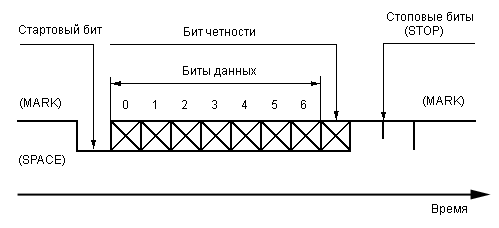
\includegraphics[scale=1.0]{phys-level}
\caption{Временная диаграмма передачи кадра.}
\label{fig:phys-level}
\end{figure}

Из рисунка видно, что исходное состояние линии последовательной передачи данных - уровень логической единицы. Это состояние линии называют отмеченным - \textbf{MARK}. Когда начинается передача данных, уровень линни переходит в логический нуль. Это состояние линии называют пустым - \textbf{SPACE}. Если линия находится в таком состоянии больше определенного времени, считается, что линия перешла в состояние разрыва связи - \textbf{BREAK}.

Стартовый бит \textbf{START} сигнализирует о начале передачи данных. Далее передаются биты данных, вначале младшие, затем старшие.

Контрольный бит формируется на основе правила, которое создается при настройке передающего и принимающего устройства. Контрольный бит может быть установлен с контролем на четность, нечетность, иметь постоянное постоянное значение логической единицы, либо отсутствовать совсем.

Если используется бит четности \textbf{P}, то передается и он. Бит четности имеет такое значение, чтобы в пакете битов общее количество единиц  (или нулей) было четно или нечетно, в зависимости от установки регистров порта. Этот бит служит для обнаружения ошибок, которые могут возникнуть при передаче данных из-за помех на линнии. Приемное устройство заново вычисляет четность данных и сравнивает результат с принятым битом четности. Если четность не совпала, то считается, что данные переданы с ошибокй. Конечно, такой алгоритм не дает стопроцентной гарантии обнаружения ошибок. Так, если при передачи данных изменилось четное число битов, то четность сохраняется, и ошибка не будет обнаружена. Поэтому на практике применяются более сложные методы обнаружения ошибок.

В самом конце передаются один или два стоповых бита \textbf{STOP}, завершающих передачу байта. Затем до прихода следующего стартового бита линия снова переходит в состояние \textbf{MARK}.

Использование бита четности, стартовых и стоповых битов определяют формат передачи данных. Очевидно, что передатчик и приемник должны использовать один и тот же формат данных, иначе обмен будет невозможен.

Другая важная характеристика - скорость передачи данных. Она также должна быть одинаковой для передатчика и приемника. Скорость передачи данных обычно измеряется в бодах. Иногда используется другой термин - биты в секунду (bps). Здесь имеется в виду эффективная скорость передачи данных, без учета служебных битов.

Интерфейс RS-232C описывает несимметричный интерфейс, работающий в режиме последовательного обмена двоичными данными. Интерфейс поддерживает как асинхронный, так и синхронный режимы работы.

Последовательная передача данных означает, что данные передаются по единственной линии. При этом биты байта данных передаются по очереди с использованием одного провода. Интерфейс называется несимметричным, если для всех цепей обмена интерфейса используется один общий возвратный провод - сигнальная <<земля>>.

\begin{center}
\begin{table}[h!]
\begin{tabular}{>{\centering}p{1.4cm}|c|c|>{\centering}p{1.3cm}}
Номер контакта & Обозначение & Назначение & Цепь 
\tabularnewline
\hline
1 & DCD (Data Carrier Detect) & Обнаружение несущей & 109 \tabularnewline
2 & RD (Receive Data)  & Принимаемые данные  & 104 \tabularnewline
3 & TD (Transmit Data) & Отправляемые данные & 103 \tabularnewline
4 & DTR (Data Terminal Ready) & Готовность терминала к работе & 108/2 \tabularnewline
5 & SG (Signal Ground) & Земля сигнала (схемная) & 102 \tabularnewline
6 & DSR (Data Set Ready) & Готовность DCE          & 107 \tabularnewline
7 & RTS (Request To Send) & Запрос передачи         & 105 \tabularnewline
8 & CTS (Clear To Send)  & Готовность DCE к приему     & 106 \tabularnewline
9 & RI (Ring Indicator)  & Индикатор вызова        & 125
\end{tabular}
\caption{Интерфейс девяти контактного разъема.}
\label{table:phys-interface}
\end{table}
\end{center}

В интерфейсе реализован биполярный потенциальный код на линиях между DTE и DCE. Напряжения сигналов в цепях обмена симметричны по отношению к уровню сигнальной <<земли>> и составляют не менее +3В для двоичного нуля и не более -3В для двоичной единицы.

Каждый байт данных сопровождается специальными сигнальными сигналами <<старт>> - стартовый бит и <<стоп>> - стоповый бит. Сигнал <<старт>> имеет продолжительность в один тактовый интервал, а сигнал <<стоп>> может длиться один, полтора или два такта.

При синхронной передаче данных через интерфейс передаются сигналы синхронизации, без которых компьютер не может правильно интерпретировать потенциальный код, поступающий по линии RD.

\subsection{Нуль-модемный интерфейс}
Обмен сигналами между адаптером компьютера и модемом (или вторым компьютером присоединенном к исходному посредством кабеля стандарта RS-232C) строится по стандартному сценарию, в котором каждый сигнал генерируется сторонами лишь после наступления определенных условий. Такая процедура обмена информацие называется запрос/ответным режимом или \textbf{<<рукопожатием>>} (\textbf{handshaking}). Большинство из приведенных в таблице сигналов как раз и нужны для аппаратной реализации <<рукопожатия>> между адаптером и модемом.

Обмен сигналами между сторонами интерфейса RS-232C выглядит так:
\begin{enumerate}
\item Компьютер после включения питания выставляет сигнал \textbf{DTR}, который постоянно удерживается активным. Если модем включен в электросеть и исправен, он отвечает компьютеру сигналом \textbf{DSR}. Этот сигнал служит подтверждением тог, что \textbf{DTR} принят, и информирует компьютер о готовности модема к приему информации;
\item Если компьютер получил сигнал \textbf{DSR} и хочет передать данные, он выставляет сигнал \textbf{RTS};
\item Если модем готов принимать данные, он отвечает сигналом \textbf{CTS}. Он служит для компьютера подтверждением того, что \textbf{RTS} получен модемом и модем готов принять данные от компьютера. С этого момента адаптер может бит за битом передавать информацию по линии \textbf{TD};
\item Получив байт данных, модем может сбросить свой сигнал \textbf{CTS}, информируя компьютер о необходимости <<притормозить>> передачу следующего байта, например, из-за переполнения внутреннего буфера; программа компьютера, обнаружив сброс \textbf{CTS}, прекращает передачу данных, ожидая повторного появления \textbf{CTS}.
\end{enumerate}

Когда модему необходимо передать данные в компьютер, модем выставляет сигнал  \textbf{DCD}. Программа компьютера, принимающая данные, обнаружив этот сигнал, читает приемный регистр, в который сдвиговый регистр <<собрал>> биты, принятые по линии приема данных \textbf{RD}. Когда для связи используются только приведенные в таблице данные, компьютер не может попросить модем <<повременить>> c передачей следующего байта. Как следствие, существует опсность переполнения помещенного ранее в приемном регистре байта данных вновь <<собранным>> байтом. Поэтому при приеме информации компьютер должен очень быстро освобождать приемный регистр адаптера. В полном наборе сигналов RS-232C есть линии, которые могут аппаратно <<приостановить>> модем.

Нуль-модемный интерфейс характерен для прямой связи компьютеров на небольшом расстоянии (длина кабеля до 15 метров). Для нормальной работы двух непосредственно соединенных компьютеров нуль-модемный кабель должен выполнять следующие соединения:
\begin{enumerate}
\item RI+DSR-1 $\leftrightarrow$ DTR-2;
\item DTR-1 $\leftrightarrow$ RI-2+DSR-2;
\item CD-1 $\leftrightarrow$ CTS-2 + RTS-2;
\item CTS-1+RTS-1 $\leftrightarrow$ CD-2;
\item RD-1 $\leftrightarrow$ TD-1;
\item TD-1 $\leftrightarrow$ RD-1;
\item SG-1 $\leftrightarrow$ SG-2;
\end{enumerate}
Знак <<+>> означает соединение соответствующих контактов на одной стороне кабеля.

\section{Настройка COM-порта средствами Haskell}
Язык Haskell имеет все нобходимые средства для работы с COM портами. Для этого необходимо установить пакет \textbf{serialport } через пакетный менеджер \textbf{cabal}. 

\subsection{Описание типов данных}
\begin{itemize}
\item \textbf{CommSpeed} - скорость передачи данных в бодах в секунду.
\begin{lstlisting}
data CommSpeed =
	CS110   |
	CS300   |
	CS600   |
	CS1200  |
	CS2400  |
	CS4800  |
	CS9600  |
	CS19200 |
	CS38400 |
	CS57600 |
	CS57600 
\end{lstlisting}
Определенные instances:
\begin{lstlisting}
Show CommSpeed
\end{lstlisting}

\item \textbf{StopBits} - количество используемых стоп битов.
\begin{lstlisting}
data StopBits =
	One |
	Two
\end{lstlisting}

\item \textbf{Parity} - тип бита четности, проверка на четность/нечетность или его отсутствие.
\begin{lstlisting}
data Parity =
	Even     |
	Odd      |
	NoParity
\end{lstlisting}

\item \textbf{FlowControl} - флаг включающий, выключающий использование возможности <<притормозить>> удаленное передающее устройство.

\begin{lstlisting}
data FlowControl =
	Software      |
	NoFlowControl
\end{lstlisting}

\item \textbf{SerialPort} - тип, инкапсулирующий открытый COM-порт.

Определенные instances:
\begin{lstlisting}
Typeable   SerialPort	 
BufferedIO SerialPort	 
RawIO      SerialPort	 
IODevice   SerialPort	
\end{lstlisting}

\item \textbf{SerialPortSettings} - настройки COM-порта.
\begin{lstlisting}
data SerialPortSettings =
	commSpeed   :: CommSpeed
	bitsPerWord :: Word8
	stopb       :: StopBits
	parity      :: Parity
	flowControl :: FlowControl
	timeout     :: Int
\end{lstlisting}
Разъяснение параметров конструктора:
\begin{itemize}
\item \textbf{commSpeed} - скорость порта в бодах в секунду;
\item \textbf{bitsPerWord} - количество битов в передаваемых словах (для асихронного режима);
\item \textbf{stopb} - количество стоп битов;
\item \textbf{parity} - тип бита четности;
\item \textbf{flowControl} - наличие контроля потока, возможность <<приостановить>> передающее устройство.
\item \textbf{timeout} - время в десятых долях секунды, после которого подвисшее соединение считается разорванным.
\end{itemize}
\end{itemize}

\subsection{Описание функций}

\begin{lstlisting}
defaultSerialSettings :: SerialPortSettings
\end{lstlisting}
Наиболее часто используемы настройки COM-порта:
\begin{itemize}
\item скорость 9600 бод в секунду;
\item в байте 8 бит;
\item 1 стоп бит;
\item без бита четности;
\item без контроля потока;
\item 0.1 секунда для timeout.
\end{itemize}

\begin{lstlisting}
setSerialSettings :: SerialPort -> SerialPortSettings -> IO SerialPort
\end{lstlisting}
Устанавливает настройки COM-порта:
\begin{itemize}
\item \textbf{SerialPort} - текущий открытый COM-порт;
\item \textbf{SerialPortSettings} - новые настройки COM-порта;
\item \textbf{IO SerialPort} - новое состояние COM-порта.
\end{itemize}

\begin{lstlisting}
getSerialSettings :: SerialPort -> SerialPortSettings
\end{lstlisting}
Получение текущих настроек COM-порта:
\begin{itemize}
\item \textbf{SerialPort} - текущий открытый COM-порт;
\item \textbf{SerialPortSettings} - настройки COM-порта;
\end{itemize}

\begin{lstlisting}
hOpenSerial :: FilePath -> SerialPortSettings -> IO Handle
\end{lstlisting}
Открывает и настраивает COM-порт, возвращает стандартный тип ссылки на устройство ввода/вывода:
\begin{itemize}
\item \textbf{FilePath} - название COM-порта, например <<COM1>> или <<COM2>>;
\item \textbf{SerialPortSettings} - первичные настройки COM-порта;
\item \textbf{Handle} - ссылка на открытый COM-порт;
\end{itemize}

\begin{lstlisting}
openSerial :: FilePath -> SerialPortSettings -> IO SerialPort
\end{lstlisting}
Открывает и настраивает COM-порт:
\begin{itemize}
\item \textbf{FilePath} - название COM-порта, например <<COM1>> или <<COM2>>;
\item \textbf{SerialPortSettings} - первичные настройки COM-порта;
\item \textbf{IO SerialPort} - новый открытый и настроенный COM-порт.
\end{itemize}

\begin{lstlisting}
closeSerial :: SerialPort -> IO ()
\end{lstlisting}
Закрывает открытый COM-порт:
\begin{itemize}
\item \textbf{SerialPort} - открытый COM-порт.
\end{itemize}

\begin{lstlisting}
withSerial :: String -> SerialPortSettings -> (SerialPort -> IO a) -> IO a
\end{lstlisting}
Безопасная функция для работы с COM-портами, закрывает порт после выполенения операции с ним:
\begin{itemize}
\item \textbf{String} - название COM-порта, например <<COM1>> или <<COM2>>;
\item \textbf{SerialPortSettings} - первичные настройки COM-порта;
\item \textbf{SerialPort -> IO a} - функция, которая будет выполнена после открытия порта;
\item \textbf{IO a} - результат выполнения функции над COM-портом.
\end{itemize}

\begin{lstlisting}
send :: SerialPort -> ByteString -> IO Int
\end{lstlisting}
Отсылает байты через COM-порт:
\begin{itemize}
\item \textbf{SerialPort} - текущий открытый COM-порт;
\item \textbf{ByteString} - буфер для отсылки;
\item \textbf{Int} - количество байтов, которое было отослано.
\end{itemize}

\begin{lstlisting}
recv :: SerialPort -> Int -> IO ByteString
\end{lstlisting}
Получение байтов из COM-порта с ограничением по количеству байтов сверху:
\begin{itemize}
\item \textbf{SerialPort} - текущий открытый COM-порт;
\item \textbf{Int} - максимальное количество байтов для приема;
\item \textbf{IO ByteString} - принятый буфер.
\end{itemize}

\begin{lstlisting}
flush :: SerialPort -> IO ()
\end{lstlisting}
Принудительно отсылает ждущие отправки данные во временных буфера COM-порта:
\begin{itemize}
\item \textbf{SerialPort} - текущий открытый COM-порт.
\end{itemize}

\begin{lstlisting}
setDTR :: SerialPort -> Bool -> IO ()
\end{lstlisting}
Устанавливает сигнал \textbf{DTR} (Data Terminal Ready) в заданное значение:
\begin{itemize}
\item \textbf{SerialPort} - текущий открытый COM-порт;
\item \textbf{Bool} - значение, которое должен принять \textbf{DTR} провод.
\end{itemize}

\begin{lstlisting}
setRTS :: SerialPort -> Bool -> IO ()
\end{lstlisting}
Устанавливает сигнал \textbf{RTS} (Ready To Send) в заданное значение:
\begin{itemize}
\item \textbf{SerialPort} - текущий открытый COM-порт;
\item \textbf{Bool} - значение, которое должен принять \textbf{RTS} провод.
\end{itemize}

\section{Канальный уровень}
\subsection{Функции канального уровня}
Канальный уровень выполняет следующие функции:
\begin{enumerate}
\item Запрос логического соединения;
\item Разбивка данных на блоки (кадры);
\item Управление передачей кадров;
\item Обеспечение необходимой последовательности блоков данных, передаваемых через межуровневый интерфейс;
\item Контроль и обработка ошибок;
\item Проверка поддержания соединения;
\item Запрос на разъединение логического соединения.
\end{enumerate}

\subsection{Протокол связи}
В основном протокол содержит набор соглашений или правил, которого должны придерживаться обе стороны связи для обеспечения получения и корректной интерпретации информации, передаваемой между двумя сторонами. Таким образом, помимо управления ошибками и потокм протокол связи регулирует также такие вопрсы, как формат передаваемых данных - число битов на каждый элемент и тип используемой схемы кодирования, тип и порядок сообщений, подлежащих обмену для обеспечения (свободной от ошибок и дубликатов) передачи информации между двумя взаимодействующими сторонами.

Перед началом передачи данных требуется установить соединение между двумя сторонами, тем самым проверяется доступность приемного устройства и его готовность воспринимать данные. Для этого передающее устройство посылает специальную команду: запрос на соединение, сопровождаемую ответом приемного устройства, например о приеме или отклонении вызова.

Также необходимо информировать пользователя о неисправностях в физическом канале, поэтому для поддержания логического соединения необходимо предусмотреть специальный кадр, который непрерывно будет посылаться с одного компьютера на другой, сигнализируя тем самым, что логическое соединение активно.

\subsection{Защита передаваемой информации}
При передаче данных по линиям могут возникать ошибки, вызванные электрическими помехами, связанными, например, с шумами, порожденными коммутирующими элементами сети. Эти помехи могут вызвать множество ошибок в цепочке последовательных битов.

Метод четности/нечетности контрольная сумма блока не обеспечивают надежного обнаружения нескольких (например, двух) ошибок. Для этих случаев чаще всего применяется альтернативный метод, основанный на полиномиальных кодах. Полиномиальные коды используются в схемах покадровой (или поблочной) передачи. Это означает, что для каждого передаваемого кадра формируется (вырабатывется) один-единственный набор контрольных разрядов, значения которых зависят от фактического содержания кадра и присоединяются передатчиком к <<хвосту>> кадра. Приемник выполняет те же вычисления с полным содержимым кадра; если при передаче ошибки не возникли, то в результате вычислений должен быть получен заранее известный ответ. Если этот ответ не совпадает с ожидаемым, то это указывает на наличие ошибок.

Опишем кратко математический аппарат циклического кодирования. Код, в котором кодовая комбинация, полученная путем циклического сдвига разрешенной кодовой комбинации является также разрешенной кодовой комбинацией называется циклическми (полиномиальным, кодом с циклическими избыточными проверками-ЦИП). Сдвиг осуществляется справа налево, при этом крайний левый символ переносится в конец комбинации. 

Циклический код относится к линейным, блочным, корректирующим, равномерным кодам. В циклических кодах кодовые комбинации представляются в виде многочленов, что позволяет свести действия надо кодовыми комбинациями к действием надо многочленами (используя аппарат полиномиальной алгебры). Циклические коды являются разновидностью систематических кодов и поэтому обладают всеми их свойствами. Первоначально они были созданы для упрощения схем кодирования и декодирования. Их эффективность при обнаружении и исправлении ошибок обеспечила им широкое применение на практике.

Циклические коды используются в ЭВМ при последовательной передаче данных. Сдвиг справа налево осуществляется путем умножения полинома на $x$. Операции сложения и вычитания выполняются по модулю 2. Они являются эквивалентными и ассоциативными. Операция деления является обычным делением многочленов, только вместо вычитания используется сложение по модулю 2.

Идея построения циклических кодов базируется на использовании непрводимых многочленов. Неприводимым называется многочлен, который не может быть представлен в виде произведения многочленов низших степеней, т.е. такой многочлен делиться только на самого себя или на единицу и не делиться ни на какой другой многочлен. На такой многочлен делиться без остатка двучлен $x^n+1$. Неприводимые многочлены в теории циклических кодов играют роль образующих полиномов.

Чтобы понять принцип построения циклического кода, умножаем комбинацию простого k-значного кода $Q(x)$ на одночлен $x^r$, а затем делим на образующий полином $P(x)$, степерь которого равна $r$. В результате умножения $Q(x)$ на $x^r$ степень каждого одночлена, входящего в $Q(x)$, повышается на $r$. ПРи делении произведения $x^rQ(x)$ на образующий полином получается частное $C(x)$ такой же степени, как и $Q(x)$. Результат можно представить в виде:
\begin{equation} \label{eq:raw-poly}
\frac{Q(x)x^r}{P(x)} = C(x) + \frac{R(x)}{P(x)}
\end{equation}
\begin{ESKDexplanation}
\item[где] $R(x)$ - остаток от деления $Q(x)x^r$ на $P(x)$.
\end{ESKDexplanation}

Частное $C(x)$ имеет такую же степень, как и кодовая комбинация $Q(x)$ простого кода, поэтому $C(x)$ ялвляется кодовой комбинацией этого же простого k-значного кода. Следует заметить, что степень остатка не может быть больше степени образующего полинома, т.е. его наивысшая степень может быть равна $(r-1)$. Следовательно, наибольшое число разрядов остатка $R(x)$ не превышает числа $r$.

Умножая обе части равенста (\ref{eq:raw-poly}) на $P(x)$ и произведя некоторые перестановки, получаем:
\begin{equation} \label{eq:made-poly}
F(x) = C(x)P(x) = Q(x)x^r + R(x)
\end{equation}

Таким образом, кодовая комбинация циклического n-значного кода может быть получена двумя способами:
\begin{enumerate}
\item умножением кодовой комбинации $Q(x)$ простого кода на одночлен $x^r$ и добавление к этому произведению остатка $R(x)$, полученного в результате деления произведения $Q(x)x^r$ на образующий полином $P(x)$;
\item умножеием кодовой комбинации $C(x)$ простого k-значного на образующий полином $P(x)$.
\end{enumerate}

При построении циклических кодов первым способом расположение информационных символов во всех комбинациях строго упорядочено - они занимают k старших разрядов комбинации, а остальные $(n-k)$ разрядов отводятся под контрольные.

При втором способе образования циклических кодов информационные и контрольные символы в комбинациях циклического кода не отделены друго от друга, что затрудняет процесс декодирования.

Как было указано выше, циклическое кодирование обладает свойством избыточности (буквально информация удваивается), и так же данный алгоритм кодирования обладает свойствами исправления ошибки в одном бите.

Алгоритм кодирования состоит в том, что каждый байт, подлежащий кодированию, разбивается на части по четыре бита, после чего делится на полином и результат деления, один байт, передается по сети, то есть, в итоге из каждого байта получается два. На принимающей стороне производится обратные операции, определяем частное и остаток. По остатку определяем вектор ошибки, если остаток нулевой, то данные дошли безошибочно, если же ненулевой, то отсылаем отрицательную квитанцию - просьбу повторить посылку пакета.

\subsection{Формат кадров}
Кадры, передаваемые с помощью функций канального уровня, имеют различное назначение. Выделены супервизорные и информационные кадры, но все кадры имеют одинаковую структуру:

\begin{table}[h!]
\begin{center}
\begin{tabular}{>{\centering}p{1.4cm}| c | >{\centering}p{2cm} | >{\centering}p{6cm}}
Номер поля & Имя поля & Размер в байтах &  Пояснение 
\tabularnewline
\hline
1 & StartByte & 1 & Стартовый байт служит для определения начала кадра. Принято значение \textit{0xFF}.
\tabularnewline
2 & Type & 1 & Тип кадра.
\tabularnewline
3 & Length & 1 & Длина поля данных, может отсутствовать для супервизорных кадров.
\tabularnewline
4 & Data & Length & Данные кадра, может отсутствовать для супервизорных кадров.
\tabularnewline
5 & StopByte & 1 & Флаг конца кадра служит для определения конца кадра. Принято значение \textit{0xFF}.
\end{tabular}
\caption{Формат кадров.}
\label{table:frame-format}
\end{center}
\end{table}

\subsubsection{Служебные супервизорные кадры}
Эти кадры используются для передачи служебной информации и реализуют следующие функции канального уровня: установление и разъединение логического канала, подтверждение приема информационного кадра без ошибок, запрос на повторную передачу принятого с ошибокй кадра. Типы этих кадров отображены в таблице~\ref{table:supervisor-frame-types}.

\begin{table}[h!]
\begin{center}
\begin{tabular}{>{\centering}p{2cm}|>{\centering}p{2cm}|>{\centering}p{4cm}|>{\centering}p{6cm}}
Поле Type & Название кадра & Описание & Данные
\tabularnewline
\hline
1 & Link & Установление соединения & Текстовый псевдоним пользователя, в ответ 
удаленная сторона присылает фрейм Option с именем собеседника.
\tabularnewline
2 & Unlink & Разрыв соединения & Отсутсвуют
\tabularnewline
3 & ACK & Потверждение безошибочного приема сообщения & Отсутствуют
\tabularnewline
4 & Ret & Запрос повторения последнего отправленного кадра & Отсутствуют
\tabularnewline
5 & Option & Изменение параметров соединения, посылается, когда пользователь с одной из сторон меняет параметры & Набор изменившихся параметров и их значения, включая псевдоним пользователя.
\end{tabular}
\caption{Формат супервизорных кадров.}
\label{table:supervisor-frame-types}
\end{center}
\end{table}

\subsubsection{Формат информационных кадров}
Информационные кадры имеют значение в поле Type равное 0, а в поле данные располагается строка для отображения в диалоге пользователя. 

\section{Прикладной уровень}
Функции прикладного уровня обеспечивают интерфейс программы с пользователем через систему форм и меню. Прикладной уровень предоставляет нижнему уровню текстовое сообщение. На данном уровне обеспечивается вывод принятых и отправленных сообщений в окно диалога пользователей.

Пользовательский интерфейс реализован на основе библиотеки \textbf{Gtk2Hs}. При его разработке в первую очередь учитывались соображения простоты, удобности и эргономичности пользовательского интерфейса.

После запуска программы пользовтель видит главное окно программы, показанное на рис.~\ref{fig:main-window}

\begin{figure}[!h]
\centering
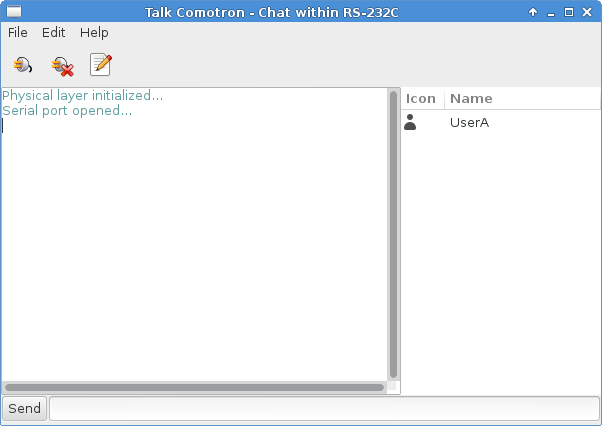
\includegraphics[scale=1.0]{main_window}
\caption{Главное окно приложения.}
\label{fig:main-window}
\end{figure}

Для настройки параметров COM-порта и своего псевдонима, пользователь может перейти к окну настроек, нажав на кнопку <<Настройки>>. Окно настроек показано на рис.~\ref{fig:options-window}.

\begin{figure}[!h]
\centering
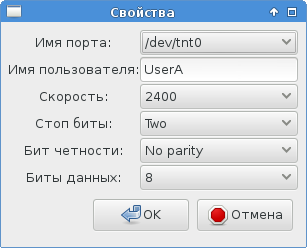
\includegraphics[scale=1.0]{options_window}
\caption{Окно настроек COM-порта.}
\label{fig:options-window}
\end{figure}

Для удобства пользователей есть возможность сохранять и загружать файлы истории, диалоги сохранения и загрузки представлены на рисункаях \ref{fig:history-save} и \ref{fig:history-load}. Диалог просмотра загруженной истории представлен на рис.~\ref{fig:history-view}. Также пользователь может получить подробную информацию о программе из диалога <<О программе>>, представленного на рис.~\ref{fig:about-dialog}.

\begin{figure}[!h]
\centering
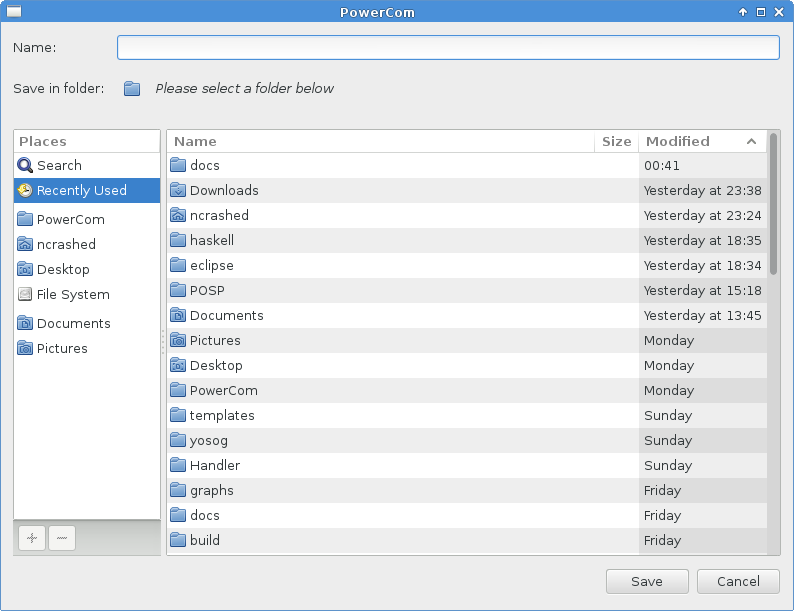
\includegraphics[width=0.8\textwidth]{history_save}
\caption{Диалог сохранения истории.}
\label{fig:history-save}
\end{figure}

\begin{figure}[!h]
\centering
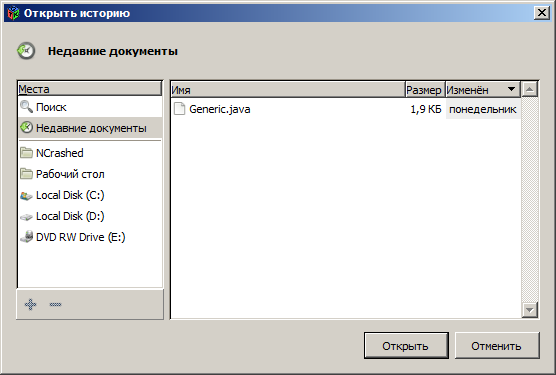
\includegraphics[width=0.8\textwidth]{history_load}
\caption{Диалог загрузки истории.}
\label{fig:history-load}
\end{figure}

\begin{figure}[!h]
\centering
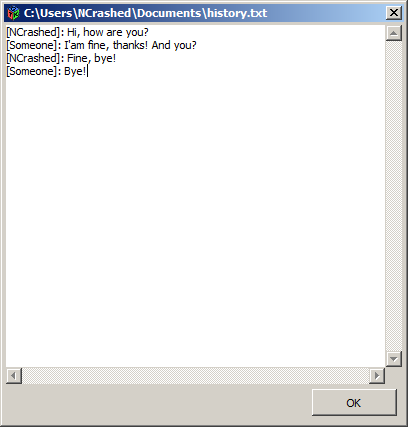
\includegraphics[width=0.6\textwidth]{history_view}
\caption{Диалог просмотра истории.}
\label{fig:history-view}
\end{figure}

\begin{figure}[!h]
\centering
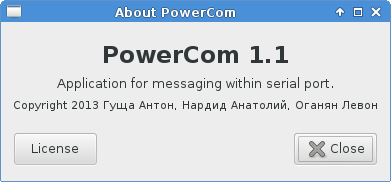
\includegraphics[scale=1.0]{about_dialog}
\caption{Диалог <<О программе>>.}
\label{fig:about-dialog}
\end{figure}

\end{document}